\documentclass[a4paper,10pt]{article}
\usepackage[utf8]{inputenc}
\usepackage{times}
\usepackage[margin=2cm]{geometry}
\usepackage{booktabs}
\usepackage{graphicx}
\usepackage{enumitem}
\usepackage{amssymb}
\usepackage{tikz}
\usetikzlibrary{arrows.meta}
\setlist{itemsep=1pt,topsep=3pt}
\newcommand{\opt}[1]{\texttt{-{}-#1}}
\newcommand{\run}[1]{\texttt{runs/#1}}

% Lab record: at most three pages. Keep the section structure.

\title{Fault-Tolerant Distributed Systems -- Lab record}
\author{Lab \textbf{2} -- Group \textbf{G}: member 1, member 2, member 3, member 4}
\date{}

\begin{document}

\maketitle
\vspace{-3em}

\section*{1. Claim}

\noindent\emph{Under assumptions} $N=3$ servers, $Q_r=Q_w=2$, lock quorum
$Q_l=2$; crash-stop failures (no recovery); asynchronous network that may
delay, reorder and drop messages (partitions) but not duplicate or corrupt
them; each client bound to one server, \emph{if at most} $f=1$ server
\emph{fails by} crashing or being cut off from the other two, \emph{the
service} (\texttt{q4b.py}) \emph{guarantees}: (i)~a read that starts after a
\texttt{write}/\texttt{cas} completed returns it or a newer value, replicas
converge, and no two \texttt{cas} succeed from the same value; (ii)~answers
to reads for clients of the live majority, and to writes/\texttt{cas}
(\emph{ok} or a definite error~11) unless the key's lock is held by the
faulty server. It does \emph{not} guarantee linearizability: a read
overlapping an unfinished write may return the new value and a later read
the old one (regular, not atomic, reads).\\
\emph{Evidence:} 19/19 linearizable runs of \texttt{q4b.py} (latency 50/rate
50, with n1 crashing, with partitions, with and without latency); each
mechanism's necessity shown by a failing run of the step before it (\S2);
the remaining anomaly reproduced (\S3).\\
\emph{Not covered:} 2 failures (no quorum); majorities-ring partitions (no
working round trip anywhere); recovery without memory; a crashed/cut-off
lock holder (key blocked forever, observed in \run{p4-crash-holder}, \run{p4-blocked-key});
fairness of the lock; valid runs are not proofs (20\,s, one hot key).

\section*{2. Design and predictions}

\noindent\textbf{Evolution} (one program per step, \texttt{code/}; every
coordinator sends to \emph{all} servers and waits for the first $Q$ answers):
\vspace{-0.3em}
\begin{center}\footnotesize
\begin{tabular}{@{}p{1.0cm}p{3.8cm}p{5.6cm}p{5.1cm}@{}}
\toprule
Part & design & what broke (run) & what we added and why \\
\midrule
1 \texttt{q1} & values only; reader returns its own copy first & 0/9 linearizable under load: concurrent writes applied in opposite orders, copies diverge (\run{p1-rowa-latency}, \run{p1-majority-latency}) & versions: servers and readers need an order on values \\
2 \texttt{q2} & \texttt{[version, value]}; writer asks a read quorum, takes max+1 & 0/5 + 2/5: concurrent writes get the \emph{same} version; each server keeps its own (\run{p2-latency}: 3 values, version 47) & tie-break on \texttt{(number, client id)}: same total order everywhere, no extra message \\
3 \texttt{q3} & tags \texttt{[n, client]} & 10/10 under load; but a read can return a write still at one server, and a later read the old value (\run{p3-inversion}, \run{p3-rowa-partition}) & kept (no write-back in Parts 1--4); fixed in ``going further'' \\
4 \texttt{q4a} & \texttt{cas} = quorum read, compare, quorum write & 0/3: two \texttt{cas(2$\to$1)} both read \texttt{[57,c11]} and both succeed (\run{p4-lost-update}) & majority lock on the key for \texttt{cas} \emph{and} \texttt{write} (2$Q_l>N$) \\
4 \texttt{q4b} & lock: refuse if held; requester releases, random backoff, error 11 after 0.8\,s & 19/19 linearizable; $\approx$3.5 locked ops/s per key; a crashed (3 of 7 crash runs) or cut-off holder blocks the key (\run{p4-crash-holder}) & (claim above) \\
+ \texttt{qx} & \texttt{q3} + write-back on reads & slow link: 0/3 $\to$ 3/3; cost: 2nd round trip, ROWA reads need all 5 (\run{px-rowa-crash}) & optional step \\
\bottomrule
\end{tabular}
\end{center}

\vspace{-0.4em}
\noindent\textbf{Part 1} (\texttt{q1.py}, 3 runs per cell; lin = linearizable runs; ok/fail/info of the first run):
\vspace{-0.3em}
\begin{center}\footnotesize
\begin{tabular}{@{}p{5.0cm}p{3.2cm}p{1.9cm}p{1.6cm}p{3.2cm}@{}}
\toprule
Config, scenario & Predicted & Observed & ok/fail/info & Why it differs \\
\midrule
ROWA (1,3) no faults / maj.\ (2,2) / non-int.\ (1,2) & lin (tiny windows); all & lin 3/3, 3/3, 3/3 & 125/81/0 & -- \\
all three, \opt{latency 50} \opt{rate 50} & NOT lin & 0/3, 0/3, 0/3 & 703/282/0 & (1,2): divergence, not stale reads \\
ROWA, n1 crashes at 5\,s & lin; no write after 5\,s & 3/3; 0 writes ok & 111/61/32 & -- \\
majority / non-int., n1 crashes & lin; all but n1's clients & 3/3, 3/3 & 118/72/7 & -- \\
ROWA, partitions & NOT lin; writes blocked & 1/3 & 138/77/3 & valid run: 2.3\,s partition \\
majority, partitions & NOT lin (stale own copy) & 3/3 & 13/139/34 & window not hit; rings block all \\
non-int., partitions & NOT lin & 0/3 & 126/80/8 & -- \\
\bottomrule
\end{tabular}
\end{center}

\vspace{-0.4em}
\noindent\textbf{Part 3, Q3} (\texttt{q3.py}, $N=5$; R/W = reads/writes still completed after the crash at 5\,s by clients of live servers):
\vspace{-0.3em}
\begin{center}\footnotesize
\begin{tabular}{@{}lllllll@{}}
\toprule
Config & no faults & n1 crashes & n1, n2 crash & partitions & msgs/op & Part 0 prediction (R / W) \\
\midrule
majority (3,3) & lin & lin; R W & lin; R W & lin & 6.56 & 2 / 2 crashes \checkmark \\
ROWA (1,5) & lin & lin; R, \textbf{no W} & lin; R, no W & \textbf{NOT lin} & 6.22 & 4 / 0 \checkmark \\
(2,4) & lin & lin; R W & lin; R, no W & lin & 6.67 & 3 / 1 \checkmark \\
(4,2) & lin & lin; R W & lin; \textbf{nothing} & lin & 6.62 & 1 / 3 \texttimes: writes 1 \\
\bottomrule
\end{tabular}
\end{center}
\vspace{-0.4em}
\noindent Our write first reads tags from $Q_r$ servers, so writes tolerate
$\min(N-Q_r,N-Q_w)$ crashes: (4,2) completes nothing with 2 crashes.
msgs/op is the same for every configuration because every request goes to
all $N-1$ others and all answer; $Q$ only sets how many answers we wait for.
\textbf{Read-heavy service: (2,4)}: reads wait for the 2 fastest of 5 and survive
3 crashes, writes survive 1; ROWA's cheaper reads cost all write
availability at the first crash or partition, and show the inversion.
\textbf{Write-heavy: majority (3,3)}: writes survive 2 crashes, the maximum;
(4,2) does not help with a two-phase write.

\section*{3. Evidence}

\run{p3-inversion} (= \texttt{store/lin-kv/20261030T152554.648Z};
\texttt{q3.py}, \texttt{SLOW\_PUT=n0=0.5}: n0's puts are held 0.5\,s;
not linearizable, key 0; reads of \texttt{q4b.py} are identical).

\begin{center}
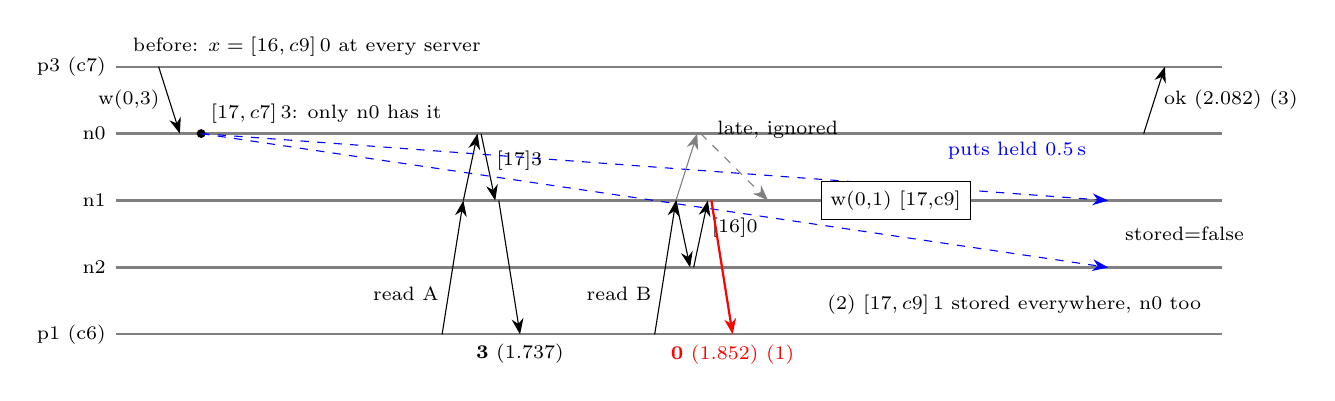
\begin{tikzpicture}[x=0.9cm,y=0.85cm,>={Stealth[length=2mm]},font=\scriptsize]
  \foreach \y/\l in {4/{p3 (c7)},3/{n0},2/{n1},1/{n2},0/{p1 (c6)}}
    \draw[thick,gray] (0,\y) node[left,black]{\l} -- (15.6,\y);
  \node[right] at (0.1,4.3) {before: $x=[16,c9]\,0$ at every server};
  % write(0,3) by p3 via n0, puts held
  \draw[->] (0.6,4) -- node[left]{w(0,3)} (0.9,3);
  \fill (1.2,3) circle (1.6pt) node[above right]{$[17,c7]\,3$: only n0 has it};
  \draw[->,dashed,blue] (1.2,3) -- (14.0,2);
  \draw[->,dashed,blue] (1.2,3) -- (14.0,1);
  \node[blue,right] at (11.6,2.75) {puts held 0.5\,s};
  % read A: n1 asks n0, gets [17]3
  \draw[->] (4.6,0) -- node[left,pos=0.3]{read A} (4.9,2);
  \draw[->] (4.9,2) -- (5.1,3);
  \draw[->] (5.15,3) -- node[right,pos=0.4]{$[17]3$} (5.35,2);
  \draw[->] (5.4,2) -- (5.7,0) node[below]{\textbf{3} (1.737)};
  % read B: n1 asks n2, gets [16]0
  \draw[->] (7.6,0) -- node[left,pos=0.3]{read B} (7.9,2);
  \draw[->] (7.9,2) -- (8.1,1);
  \draw[->] (8.15,1) -- node[right,pos=0.6]{$[16]0$} (8.35,2);
  \draw[->,red,thick] (8.4,2) -- (8.7,0) node[below]{\textbf{0} (1.852) (1)};
  \draw[->,gray] (7.9,2) -- (8.2,3);
  \draw[->,gray,dashed] (8.25,3) -- (9.2,2) node[right,black,pos=0.1,yshift=4pt]{late, ignored};
  % write(0,1) by p4 via n1
  \node[draw,fill=white] at (11.0,2) {w(0,1) [17,c9]};
  \node[right] at (9.9,0.45) {(2) $[17,c9]\,1$ stored everywhere, n0 too};
  % slow puts arrive, write ok
  \node[right] at (14.1,1.5) {stored=false};
  \draw[->] (14.5,3) -- node[right]{ok (2.082) (3)} (14.8,4);
\end{tikzpicture}
\end{center}
\vspace{-0.6em}
{\small (1)~Read B (p1, after its own read A returned 3) asks n1 and n2,
neither of which has the held put, and returns 0: \emph{new, then old}.
The error is already in A: it returned a value stored at 1 server
($<Q_w$), so a later read quorum $\{n1,n2\}$ could miss it. (2)~A
concurrent write also takes number 17 (its phase 1 asked n1, n2) and wins
the tie-break ($\texttt{c9}>\texttt{c7}$), even at n0. (3)~Write 3 completes
although its value is already gone: legal, it overlaps write 1.
\textbf{Classification} (key 0, this execution): \emph{not linearizable}: A
precedes B in real time, A needs $w(0,3)$ before it, B a write of 0 after
it, and the only one ($w(0,0)$, ended 1.492) precedes $w(0,3)$ (began
1.535). \emph{Not sequentially consistent} either: p1 read 3 then 0, while
p0 read 0 then 3 (program orders), so $w(0,0)$ must be both before and
after $w(0,3)$. With A and B by different clients and no opposite
observation, it would be sequentially consistent (order $w(0,0)$, B,
$w(0,3)$, A) but still not linearizable.}

\section*{4. Limitations and open questions}

\begin{itemize}
\item Reads are regular, not atomic (\S3); write-back fixes it
  (\texttt{qx.py}: slow link 0/3$\to$3/3) at the cost of a second round
  trip on disagreeing reads, and makes ROWA reads need all $N$ servers.
\item A lock held by a crashed or cut-off coordinator is never released:
  n1 crashed holding \{n1, n0\} (\run{p4-crash-holder}) and no lock on key~0
  was granted for the remaining 14\,s; a lock request still in flight
  from the dead n1 was granted to it in 2 more runs; a partition did the
  same (\run{p4-blocked-key}: n0, n1 got 17 error~11, 0 writes/cas).
  Next: fencing numbers / ballots so a new holder can take over safely;
  leases need clock assumptions. The lock is also unfair (starvation).
\item Not tested: recovery; $N=5$ with the lock; longer runs and many
  keys; a targeted test of \texttt{q2local}'s stale version after a heal
  (window never hit). The WSL wall clock jumped back up to 0.7\,s in some
  Part~1 runs: timelines checked against node-log order (verdicts
  unaffected).
\item The kit's \texttt{inversion-run} was not available; we reproduced
  it with a test hook (\texttt{SLOW\_PUT}) and found it naturally in ROWA
  partition runs.
\end{itemize}

\section*{5. AI log}

\begin{itemize}
\item Claude Code (Claude Opus 5.5) was asked to ``complete Lab~2'' and
  document everything: an \emph{answer directly} request, against the
  guide's think-first workflow (Part~0 and the group design questions);
  noted here and in \texttt{docs/ai-log.md}.
\item It wrote each part's design in the program header before coding and
  implemented only that design (one file per step); mechanisms it
  considered early (versions in Part~1, tie-break in Part~2, write-back,
  leases) were deferred to the part that asks for them.
\item Corrected by the runs, not by the assistant: \texttt{q2local}'s first
  valid run was not ``fewer ties'' (it had 112); no pure stale read exists
  in any Part~1 run (non-intersection shows only with partitions); crash
  and partition runs of the lock must be on top of latency.
\item \emph{(Group: add what you accepted, changed or rejected.)}
\end{itemize}

\section*{6. Contributions}

\begin{itemize}
\item member 1: \dots
\item member 2: \dots
\item member 3: \dots
\item member 4: \dots
\end{itemize}

\end{document}
